\section{Моделирование электронно-стимулированных разрывов полимерных молекул}
Количественной характеристикой процесса электронно-стимулированной деградации полимера является радиационно-химический выход разрывов $G_s$, определяемый как число разрывов молекул полимера, происходящее при выделении в нем энергии 100 эВ:
\begin{equation}
	G_s = \frac{N_{scissions}}{100 \text{ эВ}}.
\end{equation}

Экспериментально значение $G_s$ определяется на основе среднечисловых значений молекулярной массы полимера до и после экспонирования ($M_n$ и $M_f$, соответственно), определяемых методом гель-проникающей хроматографии. При известных $M_n$ и $M_f$ значение $G_s$ может быть определено из выражения~\cite{Greeneich1979_Mf_Mn}:
\begin{equation}
	{M_f = \frac{\displaystyle M_n}{1 + \frac{\displaystyle G_s E}{\displaystyle 100 \rho N_A}}}
\end{equation}

Исходя из различных экспериментов по измерению $G_s$, его значение для ПММА при экспонировании электронным лучом было принято равным 1.8~\cite{Charlesby_1964_Gs}. Также было установлено, что при экспонировании гамма- и электронным излучения при различных температурах ($T$) зависимость $\ln G_s (1/T)$ близка к линейной.

Считается, что электронно-стимулированные разрывы полимерных молекул происходят в результате взаимодействия налетающего электрона с валентными электронами атомов углерода, образующими C---C связь в главной цепи ПММА~\cite{Stepanova_2006}.

\begin{narrowfig}{G_value_exp}{G_value_exp}
	Зависимость $G_s$ от T для ПММА при экспонировании гамма- и электронным излучением.
\end{narrowfig}


\subsection{Моделирование термической деполимеризации резиста}
Термическая деполимеризация полимеров включается в себя процессы возникновения активного центра деполимеризации, его распространения вдоль молекулы полимера и последующего затухания или переноса на новую молекулу~\cite{Boyd_1}. Кинетические схемы этих процессов может быть представлена в следующем виде (обозначения $P_n$ и $R_n$ относятся к стабильной полимерной молекуле и радикализованной полимерной молекуле, соответственно, $n$ --степень полимеризации, $R_E$ -- концевой радикал):

\begin{center}
	\textbf{Возникновение активного центра деполимеризации}
	\begin{align*}
		P_n \quad \rightarrow \quad & R_r + R_{n-r} \quad & \text{случайное возникновение} \\
		P_n \quad \rightarrow \quad & R_n + R_E \quad & \text{возникновение на конце молекулы}
	\end{align*}
	\textbf{Распространение активного центра деполимеризации}
	\begin{align*}
		R_n \quad \rightarrow \quad  R_{n-1} + P_1 \qquad\qquad\qquad\qquad\quad\; \text{$P_1$ -- летучий мономер}
	\end{align*}
	\textbf{Перенос активного центра деполимеризации}
	\begin{align*}
		P_n + R_s \quad \rightarrow \quad & P_r + R_{n-r} + P_s
	\end{align*}
	\textbf{Затухание активного центра деполимеризации}
	\begin{align*}
		R_n \quad \rightarrow \quad & P_n \quad & \text{реакция 1 порядка} \\
		R_r + R_s \quad \rightarrow \quad & P_r + P_s \quad & \text{диспропорционирование} \\
		R_r + R_s \quad \rightarrow \quad & P_{r + s} \quad & \text{рекомбинация}
	\end{align*}
\end{center}

На основе данных кинетические схем можно ввести константы вышеописанных процессов и выразить скорость изменения числа стабильных полимерных молекул $P_n$ и радикализованных полимерных молекул $R_n$ за счет каждого из процессов:
\begin{center}
	\textbf{Скорость изменения числа стабильных полимерных молекул $P_n$} \\
	\textit{уменьшения $P_n$ за счет разрывов внутри молекулы:} \\
	$k_s (n-1) P_n$ \\
	\textit{уменьшения $P_n$ за счет разрывов на концах молекулы:} \\
	$k_E P_n$ \\
	\textit{уменьшения $P_n$ за счет переноса активного центра деполимеризации:} \\
	$k_I(R / V)(n-1) P_n$ \\
	\textit{увеличение $P_n$ за счет переноса активного центра деполимеризации:} \\
	{$\displaystyle k_I \frac{R_n}{V} \sum_{n=2}^{\infty} n P_n + k_{\mathrm{r}} \frac{R}{V} \sum_{j=n+1}^{\infty} P_j$} \\
	\textit{увеличение $P_n$ за счет уменьшения числа радикалов:} \\
	$k_T \alpha_n$, $\alpha_n = \left\{
	\begin{array}{l}
		R_n \quad\quad\quad\quad\quad\quad\quad\: \text{реакция 1 порядка} \\
		R_n R / V \quad\quad\quad\quad\quad\: \text{диспропорционирование} \\
		{\displaystyle \frac{1}{2} \sum_{i+j=n}^{\infty} R_i R_j / V} \quad\quad \text{рекомбинация}
	\end{array}\right.,$ \\
	где $R$ -- полное число радикалов: {$\displaystyle R = \sum_{i=1}^{\infty} R_i$} \\
	\textbf{Скорость изменения числа радикализованных полимерных молекул $R_n$} \\
	\textit{увеличение $R_n$ за счет разрывов внутри молекулы:} \\
	$2 k_S \sum_{j=n+1}^{\infty} P_j$ \\
	\textit{увеличение $R_n$ за счет разрывов на концах молекулы:} \\
	$k_E P_n$ \\
	\textit{увеличение $R_n$ за счет распространения активного центра деполимеризации:} \\
	$k_P R_{n+1}$ \\
	\textit{уменьшение $R_n$ за счет распространения активного центра деполимеризации:} \\
	$k_P R_n$ \\
	\textit{увеличение $R_n$ за счет переноса активного центра деполимеризации:} \\
	${\displaystyle k_I \frac{R}{V} \sum_{j=n+1}^{\infty} P_j}$ \\
	\textit{уменьшение $R_n$ за счет переноса активного центра деполимеризации:} \\
	${\displaystyle \frac{k_I R_n}{V} \sum_{n=2}^{\infty} n P_n}$ \\
	\textit{уменьшение $R_n$ за счет уменьшения числа радикалов:} \\
	$k_T \beta R_n$, $\beta = \left\{
	\begin{array}{l}
		1 \quad\quad\quad \text{реакция 1 порядка} \\
		R / V \quad\;\: \text{диспропорционирование или рекомбинация}
	\end{array}\right..$ \\
\end{center}

Учет всех процессов, приводящих к изменению $P_n$ и $R_n$, позволяет описать весь полимерный образец системой уравнений, описывающих каждую степень полимеризации:
\begin{equation} \label{eq:kinetic_system_original}
	\left\{
	\begin{aligned}
		&\dots \\
		&\frac{d P_n}{d t}=-(n-1)\left(k_S+k_I R / V\right) P_n-k_E P_n+k_I R / V \sum_{j=n+1}^{\infty} P_j+k_I R_n \frac{d_0}{m_0}+k_T \alpha_n \\
		&\dots \\
		&\frac{d R_n}{d t}=\left(2 k_S+k_I R / V\right) \sum_{j=n+1}^{\infty} P_j+k_E P_n-\left(\frac{k_I d_0}{m_0}+k_P+k_T \beta\right) R_n+R_P R_{n+1} \\
		&\dots \\
		&\frac{d R_1}{d t}=\left(2 k_S+k_I R / V\right) \frac{W}{x m_0}+\frac{k_E}{m_0} \frac{W}{x}-\left(\frac{k_I d_0}{m_0}+k_T \beta\right) R_1+k_P R_2,
	\end{aligned}
	\right.
\end{equation}
где $m_0$ -- масса мономера, $x$ -- среднечисловая степень полимеризации образца. 

В исходном виде система \ref{eq:kinetic_system_original} включает в себя 2$N$ уравнений ($N$ -- максимальная степень полимеризации молекул образца), и ее решение представляет собой трудоемкую задачу -- не в последнюю очередь за счет суммирования в слагаемых, описывающих эффект переноса активного центра деполимеризации на другую молекулу. Это явление является важной частью процесса полимеризации (в этом случае происходит перенос центра полимеризации)~\cite{chain_transfer_polymerization}, однако его проявление в процессе деполимеризации до сих пор находится под вопросом~\cite{Mita_PMMA_zip_lengths_T}.

Исключение процесса переноса активного центра деполимеризации из рассмотрения, а также предположение о постоянной концентрации радикализованных молекул в слое полимера существенно упрощают систему ~\ref{eq:kinetic_system_original}. В предположении о инициировании деполимеризации за счет разрывов в произвольном месте молекулы она принимает вид~\cite{Boyd_3}:
\begin{equation} \label{eq:Boyd_system_3}
	\left\{
	\begin{aligned}
		&\dots \\
		&d P_n / d t=-(n-1) k_s P_n+k_r R_n \bar{R}, \\
		&\dots \\
		&\dots \\
		&d R_n / d t=2 k_s \sum_{j=n+1}^{\infty} P_j+k_p\left(R_{n+1}-R_n\right)-k_T \bar{R} R_n=0 \quad(n \geq 2) \\
		&\dots \\
		&d R_1 / d t=2 k_s\left(W / x m_0\right)+k_p R_2-k_T \bar{R} R_1=0
	\end{aligned}
	\right.,
\end{equation}
где $\bar{R} = R/V$.

Решение системы~\ref{eq:Boyd_system_3} упрощается при условии, что распределение молекулярной массы полимера является известным. В этом случае преобразования системы приводят ее к совокупности уравнений вида~\cite{Boyd_3}:
\begin{equation} \label{eq:moment_equation}
	\frac{d M_i}{d t}=k_s\left(\frac{2}{i+1}-1\right) M_{i+1}+\frac{d M_0}{d t}-k_s M_1 - \frac{i}{\gamma}\left(k_s M_i+\frac{d M_{i-1}}{d t}\right) \quad(i \geq 1),
\end{equation}
где $1/\gamma = k_p / (k_T \bar{R})$ -- средняя длина цепи деполимеризации, $M_i$ -- момент функции распределения порядка $i$:
\begin{equation}
	M_i=\sum_{n=2}^{\infty} n^i P_n.
\end{equation}

В качестве распределения молекулярной массы полимера может использоваться распределение Шульца-Цимма~\cite{Boyd_3, Schulz-Zimm_distribution}, корректно описывающее полимеры, полученные методом радикальной полимеризации~\cite{Schulz-Zimm_distribution_proof}:
\begin{equation} \label{eq:Schulz-Zimm_distribution}
	P_n = C_0 n^z \exp (-n/y)
\end{equation}
где $P_n$ -- число молекул степени полимеризации $n$, $C_0$ -- нормировочный множитель. Параметр $z$ характеризует ширину распределения:
\begin{equation}
	M_w / M_N=(z+2) /(z+1),
\end{equation}
где $M_n$ и $M_w$ -- среднечисловая и средневесовая молекулярная масса, соответственно, а параметр $y$ определяется из выражения:
\begin{equation}
	x=y(z+1).
\end{equation}

При этом моменты функции распределения высших порядков могут быть выражены через параметры $y$ и $z$ и момент первого порядка $M_1$:
\begin{equation}
	M_i=M_1 \prod_{n=2}^i(z+n) y^{i-1}.
\end{equation}
Отметим, что $M_0$ выражает полное число полимерных молекул, $M_1$ -- среднечисловую степень полимеризации.

Далее удобно ввести безразмерные переменные:
\begin{equation}
	\begin{aligned}
		\tau & = y^0 k_s t \\
		\tilde{M}_1 & = M_1 / M_1^0 \\
		\tilde{y} & = y / y^0 \\
		\tilde{\gamma} & = \gamma y^0 \\
		\tilde{x} & = x / x^0 = \left[y(z+1) / y^0\left(z^0+1\right)\right],
	\end{aligned}
\end{equation}
которые в дальнейшем используются в уравнениях вида~\ref{eq:moment_equation} для $i$, равного 1, 2 и 3. В конечном счете система этих трех нелинейных дифференциальных уравнений первого порядка принимает вид:

\begin{equation} \label{eq:scary_system}
	\begin{aligned}
		&\frac{\tilde{M_1}^{\prime}}{\tilde{M_1}}=\left[\frac{1}{\tilde{y}} \frac{d \tilde{y}}{d \tau}+\frac{1}{(z+1)} \frac{d z}{d \tau}-\tilde{y}(z+1)\right] /[1+\tilde{\gamma} \tilde{y}(z+1)] \\
		&\tilde{y}^{\prime}=(B F-C E) /(A E-D B) \\
		&z^{\prime}=(C D-A F) /(A E-D B),
	\end{aligned}
\end{equation}
где
\begin{equation}
	\begin{aligned}
		&A=-\left[\frac{1}{\tilde{y}[1+\tilde{\gamma} \tilde{y}(z+1)]}+\frac{(z+2) \tilde{\gamma}}{(z+2) \tilde{\gamma} \tilde{y}+2}\right] \\
		&B=-\left[\frac{1}{(z+1)[1+\tilde{\gamma} \tilde{y}(z+1)]}+\frac{\tilde{\gamma} \tilde{y}}{(z+2) \tilde{\gamma} \tilde{y}+2}\right] \\
		&C=\left[\frac{\tilde{y}(z+1)}{\tilde{\gamma} \tilde{y}(z+1)+1}-\frac{\frac{1}{3}(z+2)(z+3) \tilde{\gamma} \tilde{y}^2+2(z+2) \tilde{y}}{(z+2) \tilde{\gamma} \tilde{y}+2}\right] \\
		&D=\left[\frac{(z+2) \tilde{\gamma}}{(z+2) \tilde{\gamma} \tilde{y}+2}-\frac{2(z+2)(z+3) \tilde{\gamma} \tilde{y}+3(z+2)}{(z+2)(z+3) \tilde{\gamma} \tilde{y}^2+3(z+2) \tilde{y}}\right] \\
		&E=\left[\frac{\tilde{\gamma} \tilde{y}}{(z+2) \tilde{\gamma} y+2}-\frac{\tilde{\gamma} \tilde{y}(2 z+5)+3}{(z+2)(z+3) \tilde{\gamma} \tilde{y}+3(z+2)}\right] \\
		&F=\left[\frac{\frac{1}{3}(z+2)(z+3) \tilde{\gamma} \tilde{y}^2+2(z+2) \tilde{y}}{(z+2) \tilde{\gamma} \tilde{y}+2}-\right. \\
		&\left.-\frac{\frac{1}{2}(z+2)(z+3)(z+4)\left(\tilde{\gamma} \tilde{y}^2+3(z+2)(z+3) \tilde{y}\right.}{(z+2)(z+3) \tilde{\gamma} \tilde{y}+3(z+2)}\right].
	\end{aligned}
\end{equation}
Производные в левой части~\ref{eq:scary_system} берутся по переменной $\tau$, а сама система решается численно.


\section{Моделирование термического растекания резиста}

\subsection{Аналитический подход}
Моделирование оплавления резиста может быть проведено аналитически на основе подхода, предложенного для моделирования оплавления периодических структур, полученных методом НИЛ~\cite{Leveder_2008, Leveder_2011}. В его основе лежит Фурье-преобразование профиля резиста $h(t)$:
\begin{equation}
	\begin{aligned}
		& h(x, t) = h_0 + \tilde{h}(x, t) \\
		& \tilde{h}(x, t) = \sum_{-\infty}^{+\infty} a_n(t) \exp \left(i n \frac{2 \pi}{\lambda} x\right),
	\end{aligned}
\end{equation}
где $h_0$ -- средняя высота профиля, $\lambda$ -- пространственный период профиля.

Уравнения Навье-Стокса при условии отсутствия проскальзывания и с учетом расклинивающего и Лапласова давления может быть выражено в виде:
\begin{equation}
	\partial_t \tilde{h}-\frac{A}{6 \pi \eta h_0} \partial_x^2 \tilde{h}+\frac{\gamma h_0^3}{3 \eta} \partial_x^4 \tilde{h} = 0,
\end{equation}
где $A$ -- постоянная Гамакера, $\gamma$ -- коэффициент поверхностного натяжения резиста.

Его решение приводит к выражению для времени затухания $n$-й гармоники профиля $\tau_n$:
\begin{equation}
	\frac{1}{\tau_n}=\left(n \frac{2 \pi}{\lambda}\right)^2 \frac{A}{6 \pi h_0 \eta}+\left(n \frac{2 \pi}{\lambda}\right)^4 \frac{\gamma h_0^3}{3 \eta}.
\end{equation}

При выполнении условия $\left(\frac{\displaystyle h_0^2}{\displaystyle \lambda}\right)^2 \ll \frac{\displaystyle A}{\displaystyle \gamma}$ выражение для $\tau_n$ принимает более простой вид:
\begin{equation}
	\tau_n=\frac{3 \eta}{\gamma h_0^3} \times\left(\frac{\lambda}{2 \pi n}\right)^4.
\end{equation}

Результирующий профиль в момент времени $t$ определяется суммой гармоник:
\begin{equation}
	\tilde{h}(x, t)=\sum_{-\infty}^{+\infty} a_n(0) \exp \left(-\frac{t}{\tau_n}+i n \frac{2 \pi}{\lambda} x\right).
\end{equation}


\begin{figure}
	\begin{minipage}{0.5\textwidth}
		\raggedright
		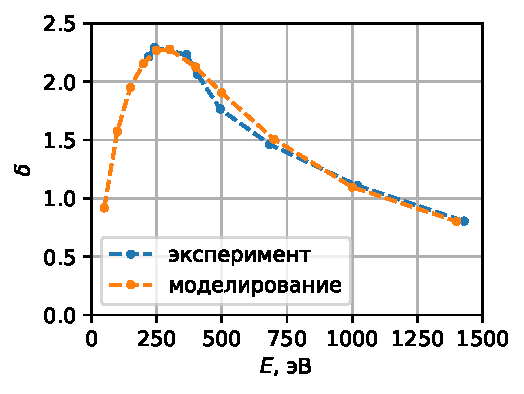
\includegraphics{pdf/2ndary_yield_1p9}
	\end{minipage}%\hfill
	\begin{minipage}{0.5\textwidth}
		\raggedleft
		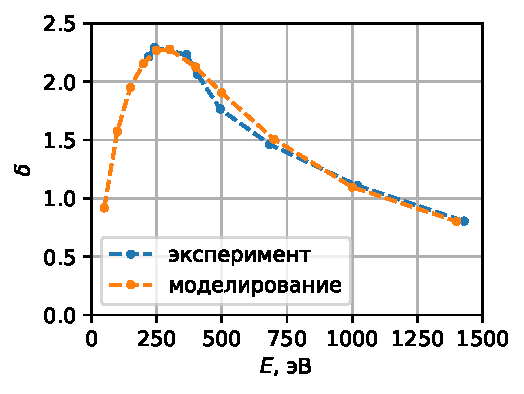
\includegraphics{pdf/2ndary_yield_1p9}
	\end{minipage}%\hfill
	\caption{An example graph}
\end{figure}


\begin{figure}
	\begin{minipage}{0.5\textwidth}
		\raggedright
		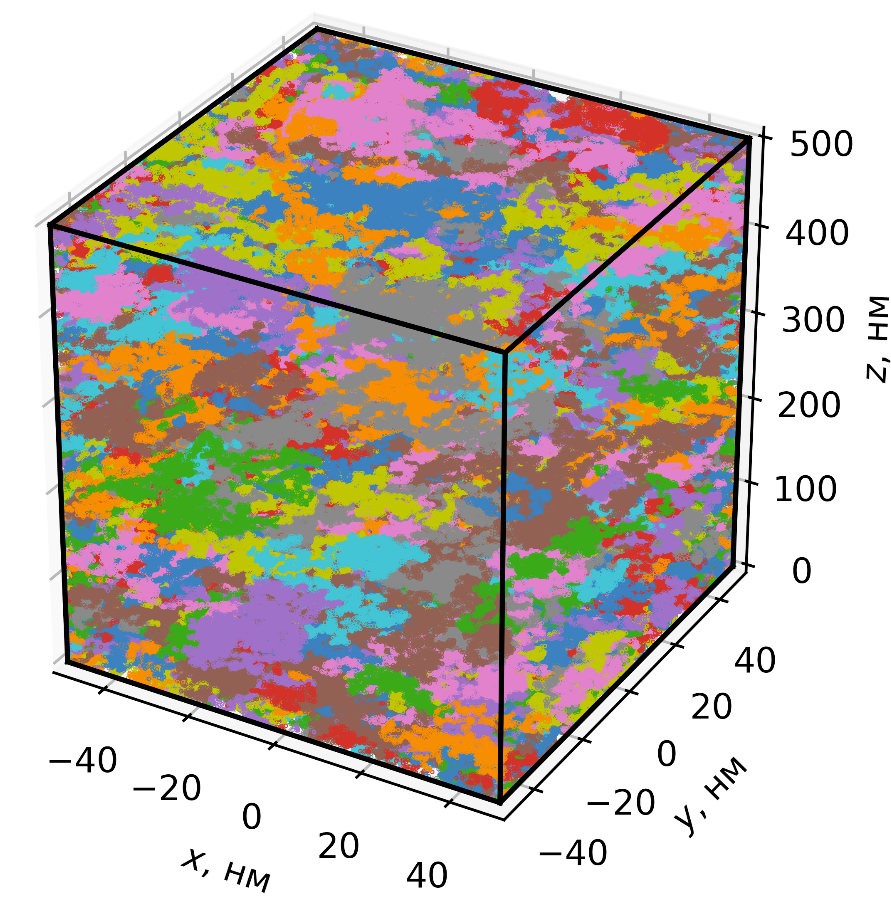
\includegraphics{jpg/Harris_chains}
	\end{minipage}%\hfill
	\begin{minipage}{0.5\textwidth}
		\raggedleft
		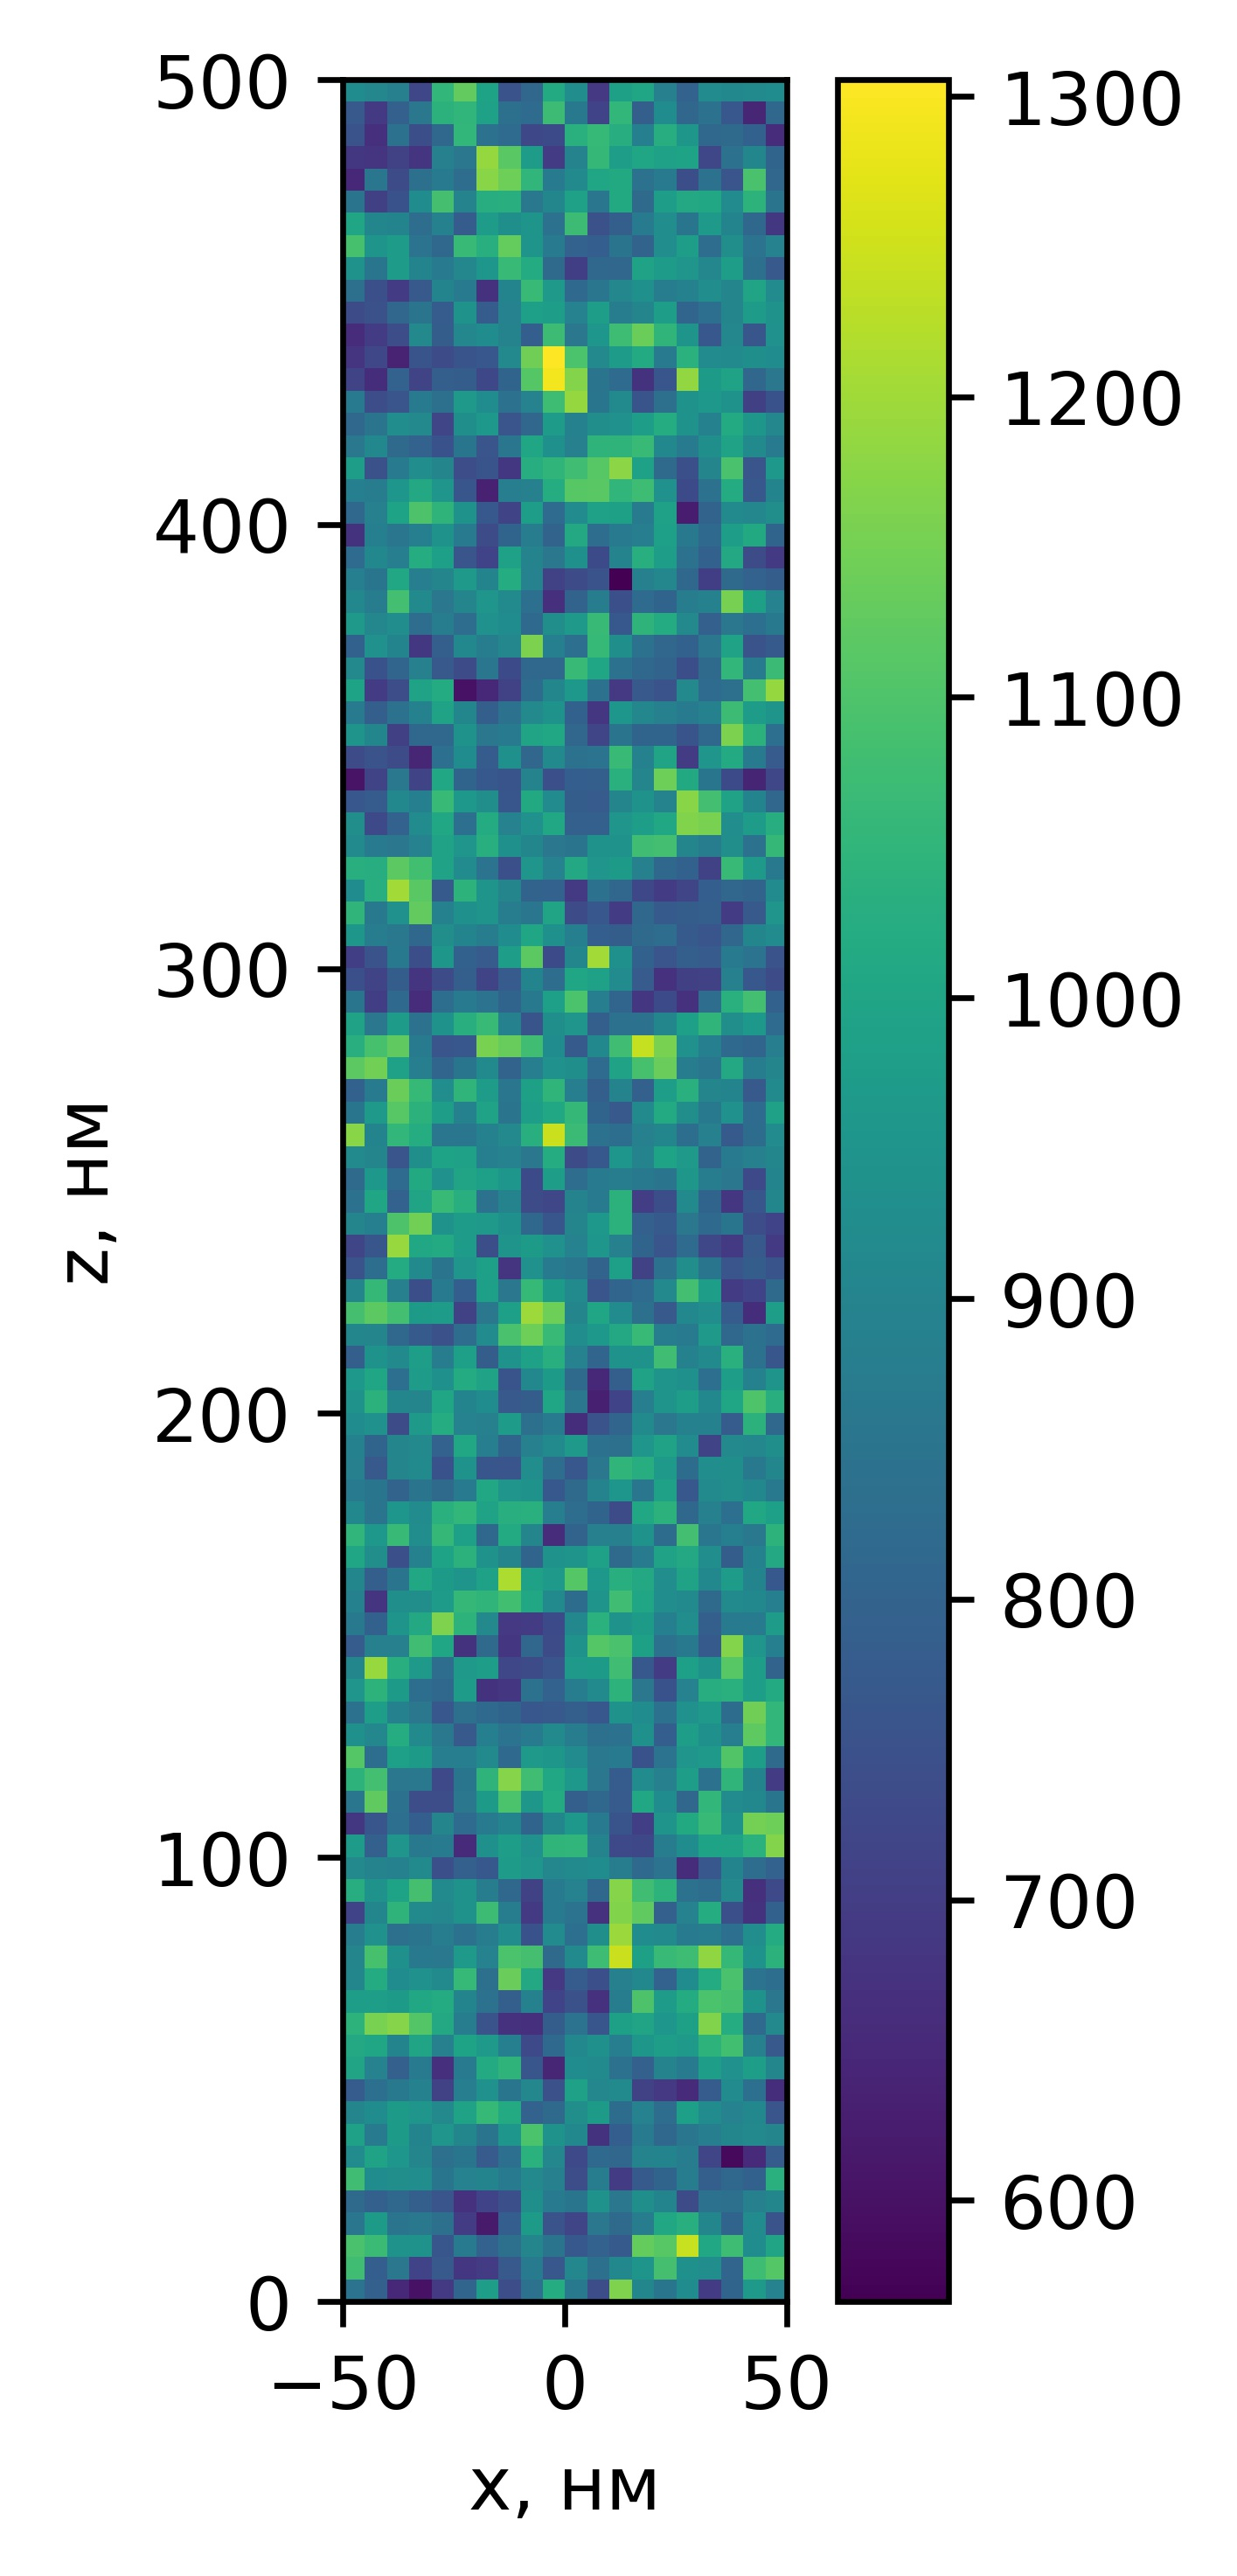
\includegraphics{jpg/Harris_hist_5nm}
	\end{minipage}%\hfill
	\caption{An example graph}
\end{figure}


\subsection{Численный подход}







